\chapter{Sistemas de almacenamiento}

\section{Introducción}

En este primer capítulo se presentan de forma general los sistemas de almacenamiento utilizados en este trabajo: los supercapacitores y las baterías de litio. Se analizan sus principios de funcionamiento, distintas clasificaciones que existen de ambas (junto con sus diferencias constructivas) y las aplicaciones que poseen. Finalmente, se realiza una comparación entre ambos sistemas de almacenamiento en base a sus capacidades de almacenar energía y la rapidez con la que pueden entregarla. 

Los supercapacitores son dispositivos de alta densidad másica de energía comparados con los capacitores electrolíticos convencionales, y pueden llegar a capacitancias de hasta \SI{5000}{\farad}. Para aplicaciones en donde se necesita una cantidad de energía significativa en forma de pulso, los capacitores tradiciones utilizados en circuitos electrónicos son incapaces de almacenar o entregar tal cantidad en el volumen y peso disponible. Estos dispositivos son utilizados en aplicaciones que demandan estas propiedades, tales como en el freno regenerativo o en la aceleración de vehículos.

Las baterías de ión de litio, también llamadas baterías Li-Ion, son un tipo de baterías recargables compuestas por celdas en las que los iones de litio se transfieren desde un electrodo negativo a uno positivo a través de un electrolito al ser descargadas, y viceversa al cargarse.  Este tipo de baterías poseen una gran densidad másica de energía, no poseen memoria\footnote{La disminución de la energía utilizable, en relación a la almacenable, a lo largo de los ciclos de carga y descarga.}, y su autodescarga es muy baja.

\section{Supercapacitores}

\subsection{Clasificación y principio básico de funcionamiento}

Debido a que existen distintos tipos de supercapacitores (clasificados por la forma de almacenar carga), las capacidades intrínsecas de estos dispositivos, mencionadas en la introducción de este capítulo, se dan de distinta manera en cada tipo de supercapacitor:

\begin{itemize}
    \item Los \textbf{supercapacitores de doble capa electroestática (EDLCs)} almacenan carga electroestáticamente en una doble capa formada cerca de la interfaz electrodo-electrolito, y pueden ser cargados y descargados hasta 10$^6$ veces sin pérdida de densidad másica de potencia. Utilizan electrodos de carbono o derivados con un alto grado de porosidad, lo que se traduce a un aumento importante en su área efectiva, y por ende logran una alta capacitancia.
    \item Los \textbf{pseudocapacitores electroquímicos} almacenan carga electroquímicamente vía inserción y absorción de los iones del electrolito a la superficie del electrodo junto a reacciones reducción-oxidación (redox) del almacenamiento de carga. Están construidos con electrodos de óxido o polímero conductor y su almacenamiento de cargas depende de los enlaces químicos que se generan entre el electrodo y el electrolito.
    \item Los \textbf{supercapacitores híbridos} combinan estas dos características y presentan tanto efectos pseudocapacitivos como electroestáticos.
\end{itemize}

\begin{figure}[hbt!]
  \centering
  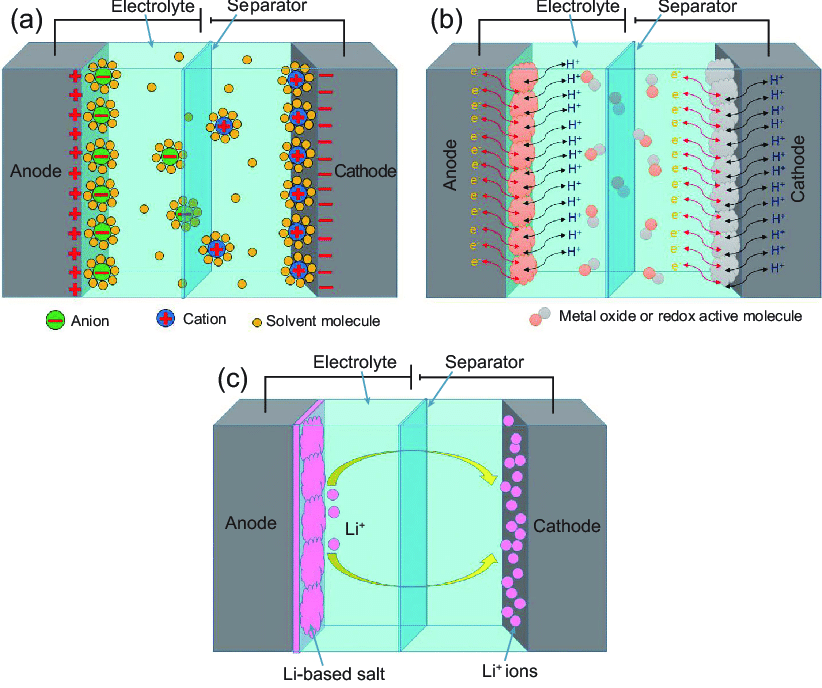
\includegraphics[width=0.50\columnwidth]{Imágenes/Diagrama esquemático de supercapacitores.png}
  \caption{Diagramas esquemático de los distintos tipos de supercapacitores. (a) EDLC (b) Pseudocapacitor (c) Híbrido.}
  \label{ragone}
\end{figure} 


\subsection{Aplicaciones}

Los supercapacitores son deseados en aplicaciones en donde es necesaria una gran cantidad de potencia en una ventana de tiempo pequeña. Algunos ejemplos de estas aplicaciones son:

\subsubsection{Búfer de energía para equipos de baja potencia}

Los supercapacitores pueden utilizarse como una fuente de energía de respaldo para RAM, SRAM y microcontroladores en el caso de un apagado de emergencia. Las UPS (del inglés \emph{uninterruptible power supplies}, sistemas de alimentación ininterrumpida) pueden ser alimentadas por supercapacitores, los cuales reemplazarían bancos de capacitores electrolíticos con mayores dimensiones físicas, y poseen un menor costo por ciclo, entre otras características que favorecen económicamente el uso de estos dispositivos.

\subsubsection{Microrredes}

Debido a que las microrredes generalmente son alimentadas con energía limpia y renovable, su producción no es constante a lo largo del día, y puede no llegar a igualar la demanda. El rol de los supercapacitores en una microrred en estos casos sería inyectar potencia en forma casi instantánea cuando la demanda es alta y la producción es baja. En esta situación, los supercapacitores actúan de forma óptima como búfer en conjunto con baterías químicas (como por ejemplo, baterías de litio).

En toda|s estas aplicaciones y debido a sus bajos niveles de tensión, los supercapacitores son utilizados en \emph{arreglos} o \emph{bancos} para poder satisfacer los requerimientos de cada aplicación, los cuales pueden ser de tensión, corriente o energía eléctrica.

\subsection{Bancos de supercapacitores}

Un banco de supercapacitores se define como un arreglo de supercapacitores, agrupados de forma de poder ser incluidos en sistemas de mayor potencia, y satisfacer ciertos requerimientos que un solo supercapacitor no podría cumplir. Observando las ecuaciones de capacidad equivalente para distintos arreglos:

\begin{itemize}
  \item Capacitor equivalente en serie:
  \begin{equation}
    \frac{1}{C_{eq}} = \sum_{n=1}^{N} \frac{1}{C_i}
    \label{cap-serie}
  \end{equation}
  \item Capacitor equivalente en paralelo:
  \begin{equation}
    C_{eq} = \sum_{n=1}^{N} C_i
    \label{cap-paralelo}
  \end{equation}
\end{itemize}

Dado que los valores de tensión que se manejan en sistemas de potencia son más elevados que los valores de tensión nominales de un solo supercapacitor, se coloca el número de elementos en serie que sea necesario hasta alcanzar el nivel de tensión requerido. Debido a que esto conlleva una disminución de la capacitancia del sistema, como puede observarse en la Ecuación \ref{cap-serie} el arreglo utilizado para este trabajo consiste en un arreglo conformado por celdas tanto en paralelo como en serie para contrarrestar este efecto indeseado \cite{fornaro}.

\subsubsection{Inconvenientes}

En supercapacitores que presentan elevados valores de capacidad, pequeños valores de tolerancia representan grandes variaciones de energía, y dentro de un mismo sistema, estas ligeras variaciones pueden significar la ruptura del material que aísla las cargas en un supercapacitor.

Uno de los primeros efectos que puede verse en un supercapacitor que trabaja por encima de su valor nominal es la evaporación interna de los materiales que componen el electrolito, generando un aumento de la presión dentro del dispositivo capaz de provocar un estallido, destruyendo el encapsulado y poniendo el riesgo la salud del operario. Para esto es necesario conocer los valores a los cuales trabajarán en un determinado sistema tanto el banco completo de supercapacitores como cada supercapacitor individualmente, y tener dichos valores controlados en pos de un sistema eficiente y seguro.

Es por este motivo que en el diseño del banco de supercapacitores se debe implementar un método de control en las tensiones de cada celda, ya que si nos encontramos con que una de las celdas tiene un bajo valor de capacidad respecto de las otras, éstas tendrán un alto valor de tensión en estado estacionario pudiendo sobrepasar la tolerancia máxima, culminando en la destrucción del sistema completo. 

El banco de supercapacitores disponible en el instituto, y utilizado en este trabajo, posee un esquema de balanceo empleando transistores MOSFET, el cual es explicado a continuación.

\subsubsection{Método de balanceo mediante MOSFET}

Este control supone emplear las llaves MOSFET colocadas en paralelo con cada juego de supercapacitores. Las mismas aumentan su corriente exponencialmente a medida que aumenta la tensión del supercapacitor. En la Figura \ref{balanceo-mosfet} puede observarse un diagrama del método.

Tiene un manejo más eficiente de la energía, debido a que con baja tensión en el supercapacitor, los valores de corriente a través de la llave son extremadamente bajos, y al llegar el supercapacitor a un estado de carga determinado, los valores de corriente a través de la llave contribuyen para ir progresivamente balanceando el conjunto de celdas, y llegar al estado de carga sin tener que descargar elevados valores de corriente.

\begin{figure}[hbt!]
  \centering
  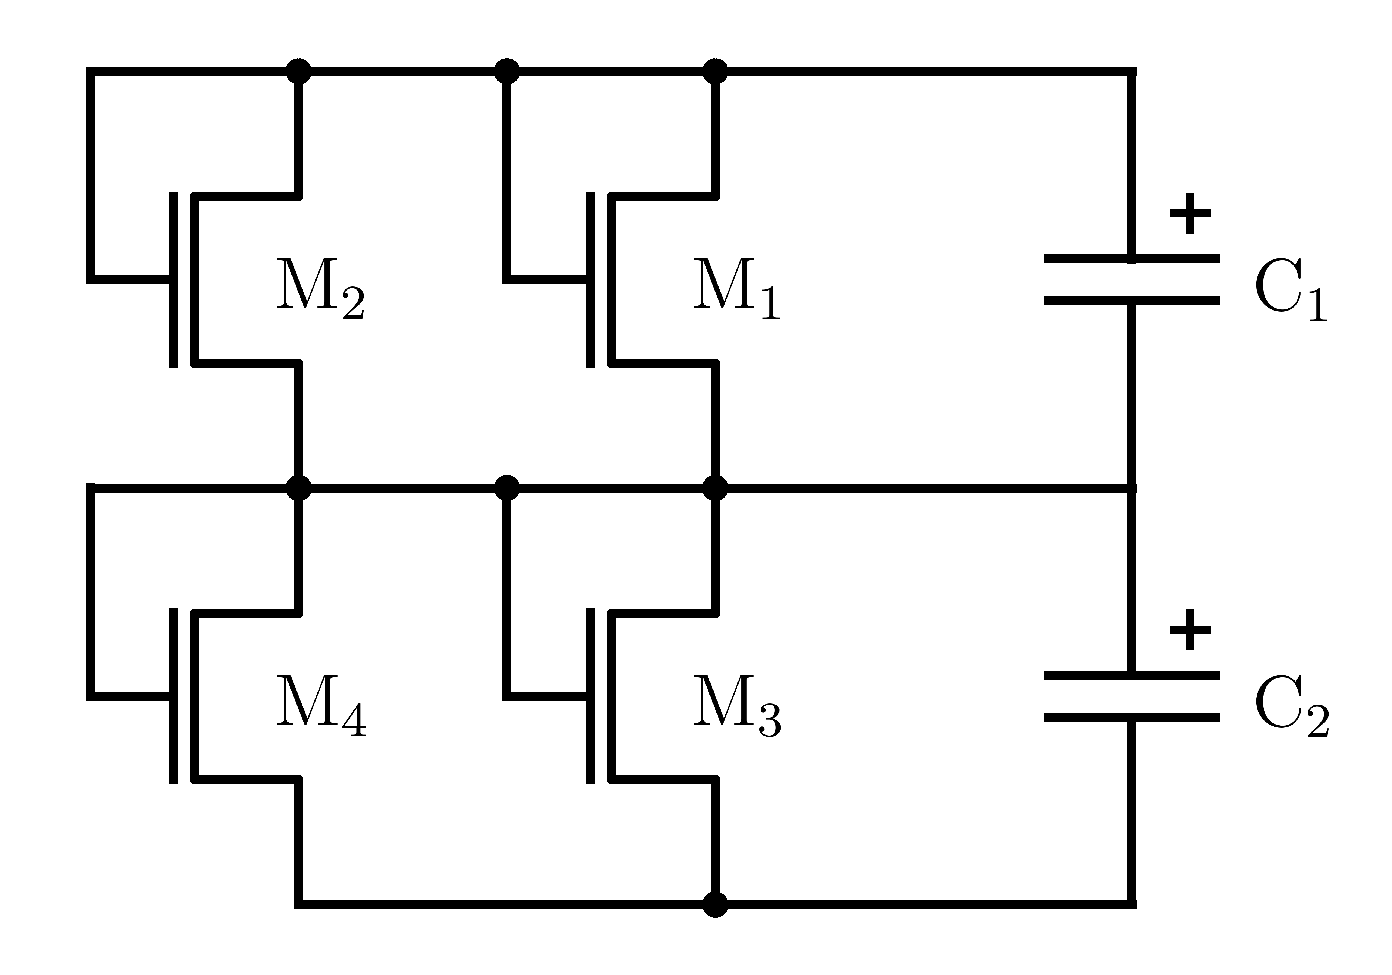
\includegraphics[width=0.40\columnwidth]{Imágenes/Balanceo por MOSFET.pdf}
  \caption{Diagrama circuital del balanceo mediante MOSFET.}
  \label{balanceo-mosfet}
\end{figure} 

En resumen, este método emplea MOSFET como resistencias variables para balancear los supercapacitores. De esta forma, si algún supercapacitor comienza a elevar su tensión respecto del resto de los elementos del banco, entonces su resistencia de descarga será menor, compensando selectivamente las diferencias en el banco.

\section{Baterías de ión de litio}

\subsection{Principio básico de funcionamiento}

Los reactivos en las reacciones electroquímicas de una celda de Li-Ión son el ánodo y cátodo, los cuales contienen átomos de litio. Durante la carga, iones $\text{Li}^+$ son generados por el electrodo positivo (el cual funciona como ánodo en este proceso), migran a través del electrolito y el separador poroso, y penetran el electrodo negativo (el cual funciona como cátodo), mientras los electrones circulan por el circuito externo. En el proceso, el electrodo positivo se oxida perdiendo electrones, y el electrodo negativo es reducido (reacción \emph{redox}) capturando electrones.

\subsection{Características constructivas}

La gran ventaja de la tecnología de litio proviene del hecho de que Li es un metal liviano, y es el elemento más electropositivo\footnote{La tendencia de un átomo de donar electrones y formar cationes positivamente cargados.} que se encuentra en la naturaleza (lo que hace que la tensión de sus baterías sea significativamente más alta que la de otras tecnologías). Además las baterías de Li-Ión son de bajo mantenimiento, lo cual es una ventaja que otros tipos de tecnología, como por ejemplo las baterías a base de níquel, no poseen. Las baterías de ión de litio pueden usar diferentes materiales como electrodos:

\begin{itemize}
  \item La combinación más común es un cátodo de \textbf{óxido de litio cobalto} y un ánodo de \textbf{grafito}, utilizado mayormente en dispositivos electrónicos portables como celulares y notebooks.
  \item Otros materiales utilizados para el cátodo se tratan de \textbf{dióxido de litio-manganeso}, utilizado en automóviles híbridos y eléctricos, y \textbf{litio-ferrofosfato}.
\end{itemize}

Las baterias de litio utilizan ésteres (un tipo de compuesto orgánico) como electrolito. En el instituto se encuentran disponibles baterías de litio-ferrofosfato, las cuales se describen de forma más extensa a continuación.

\begin{figure}[hbt!]
  \centering
  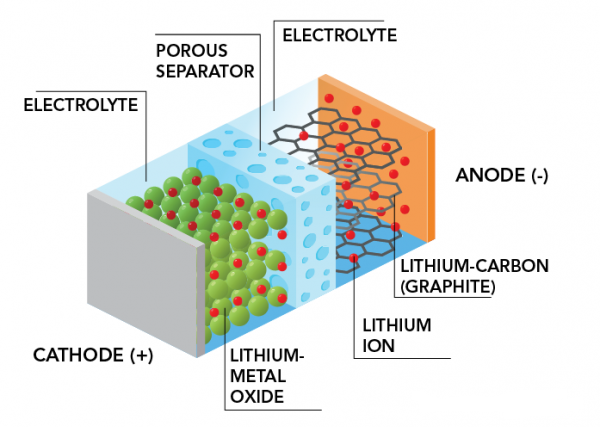
\includegraphics[width=0.47\columnwidth]{Imágenes/Partes de una batería.png}
  \caption{Partes de una batería de ión-litio.}
  \label{bateria}
\end{figure} 

\subsection{Baterías de litio-ferrofosfato}

Las baterías de litio-ferrofosfato (LiFePO$_4$ o LFP) son un tipo de baterías de Li-Ión que utilizan litio-ferrofosfato como material de cátodo, y grafito con respaldo metálico como ánodo. La densidad másica de energía en una batería LFP es menor que la de otros tipos de baterías Li-Ión, y también posee una tensión nominal menor. Aún así, debido a su bajo costo, baja toxicidad (no posee cobalto), largo ciclo de vida y otros factores, las baterías LFP se están utilizando cada vez más en vehículos, aplicaciones estacionarias a gran escala, y sistemas de energía de emergencia.

Un ejemplo de este emergente uso de las baterías LFP se da en una de las empresas automotoras y de energía limpia más novedosas del mundo, \emph{Tesla}, la cual anunció que cambiará las baterías de óxido de níquel-cobalto-aluminio (NCA), utilizadas en sus vehículos y aplicaciones estacionarias (como por ejemplo, el \emph{Megapack} de la Figura \ref{megapack}), por este tipo de tecnología.

\begin{figure}[hbt!]
  \centering
  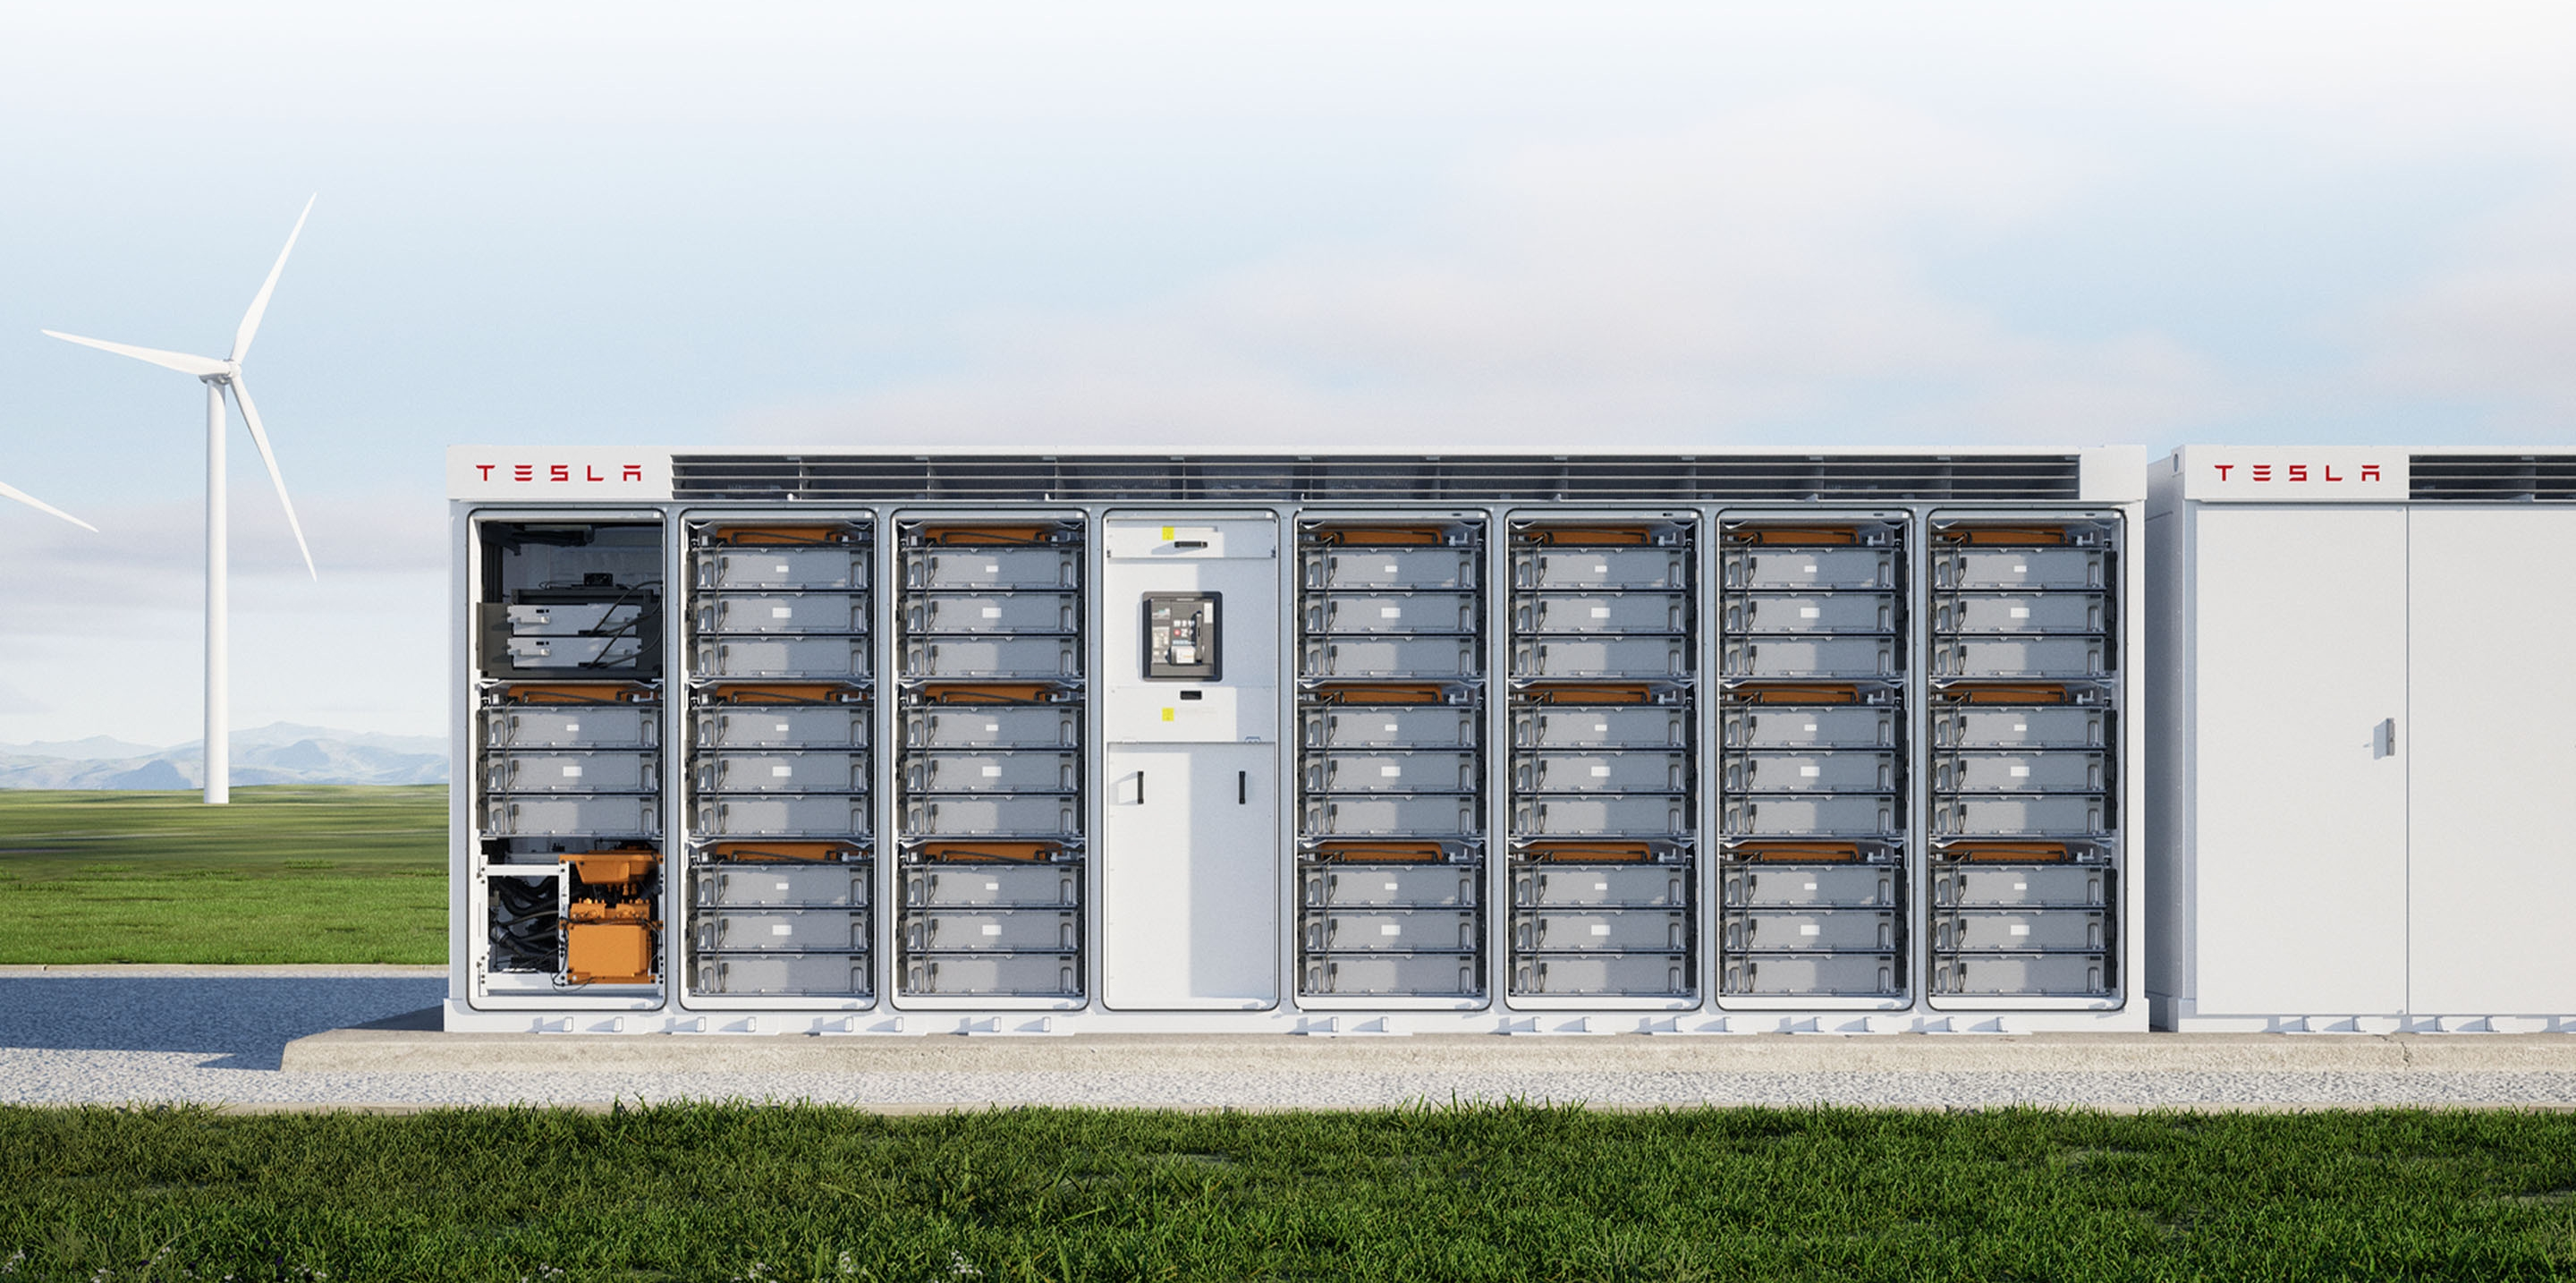
\includegraphics[width=0.65\columnwidth]{Imágenes/Tesla Megapack.jpg}
  \caption{Megapack de Tesla, un producto estacionario de almacenamiento de energía a gran escala.}
  \label{megapack}
\end{figure} 

\subsection{Proceso de carga y descarga}

El proceso de carga para una batería de Li-Ión, la cual está compuesta de un grupo de celdas en serie, se divide en tres etapas:

\begin{enumerate}
  \item Durante la etapa de \textbf{corriente constante} (CC), el cargador aplica una corriente continua a la batería, con una tensión con tasa de aumento constante, hasta que el límite de tensión por celda es alcanzado.
  \item En la etapa de \textbf{balanceo}, el cargador reduce la corriente de carga mientras que el estado de carga (siglas SoC, del inglés \emph{state of charge}) de las celdas individuales es llevado al mismo nivel por el circuito de balanceo, llamado BMS (del inglés \emph{battery management system}). Las técnicas para lograr este balanceo varían de cargador en cargador.
  \item Finalmente, en la fase de \textbf{tensión constante}, el cargador aplica un voltaje igual a la tensión nominal de las celdas multiplicado por la cantidad de celdas en series que posee la batería, mientras la corriente disminuye gradualmente hacia cero hasta un cierto umbral especificado por el cargador. 
\end{enumerate}

El electrolito y el circuito externo proveen conducción de los elementos, pero no participan de la reacción electroquímica.

Durante la descarga, los electrones fluyen desde el electrodo negativo (ánodo) hacia el electrodo positivo (cátodo) a través del circuito externo. La reacción durante la descarga reduce el potencial químico de la celda, y por lo tanto este proceso transfiere energía de la celda a donde se disipe la energía (en gran parte el circuito externo).

Ambos electrodos permiten a estos iones de litio entrar y salir de sus estructuras a través de un proceso llamado \emph{inserción}\footnote{La inserción, también llamada intercalación, es la inclusión reversible de una molécula o ión en materiales con estructura laminar o en capas.} o \emph{extracción}, respectivamente. En la Figura \ref{bateria} puede observarse la estructura de una batería de Li-Ion, en donde se identifican el cátodo, ánodo, electrolito, y el separador poroso.

\subsection{Aplicaciones}

\subsubsection{Autos eléctricos}

La electrificación de los vehículos esta aumentando a una tasa cada vez más rápida, debido a que existen varias ventajas en utilizar trenes motrices eléctricos, comparado con los motores de combustion interna, para aplicaciones automóviles. La primer ventaja es que los dispositivos eléctricos pueden alcanzar una eficiencia de energía mucho más alta que los motores de combustión interna. La segunda ventaja es un derivado del \emph{freno regenerativo} en donde una batería recargable es instalada en un sistema, y almacena energía cinética convirtiéndola en energía eléctrica, aumentando la eficiencia \cite{evs&hevs}.

Además, estos sistemas eléctricos pueden aprovechar un gran abanico de fuentes de energía, desde centrales termoeléctricas, hasta tecnologías de energía renovable como celdas fotovoltáicas o turbinas eólicas (Figura \ref{hev}).

\begin{figure}[hbt!]
  \centering
  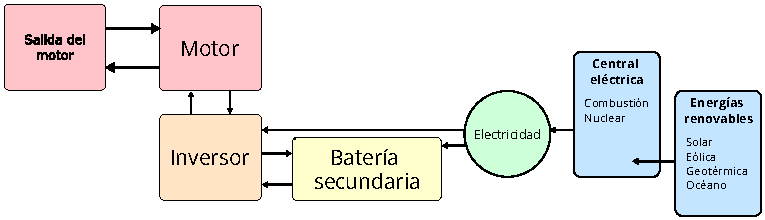
\includegraphics[width=0.65\columnwidth]{Imágenes/Flujo de la energía en un HEV.pdf}
  \caption{Flujo de la energía en un vehículo eléctrico.}
  \label{hev}
\end{figure}

\subsubsection{Almacenamiento de energías renovables}

Este tipo de baterías también puede ser utilizadas para solucionar el problema de la fluctuación de fuentes de energías renovables, como la energía solar o eólica. Además de la extensión de la red eléctrica y el desarrollo de soluciónes de gestión del lado de la demanda, el almacenamiento de energía es crucial para lograr un sistema eléctrico basado principalmente en energías renovables \cite{storage}. 

Un ejemplo de esta situación se da en Alemania. En 2011, las energías renovables ya aportaban aproximadamente el 20\% de la producción de energía eléctrica. En 2012, los sistemas fotovoltáicos lograron en los primeros seis meses una participación del 5.1\%, mientras que los generadores éolicos una participación del 8.9\% de la energía eléctrica total producida. Los primeros días de agosto del 2012, la energía solar alcanzó una producción de \SI{31}{\giga\watt} sobre la capacidad instalada, y la energía eólica un valor de más de \SI{29}{\giga\watt}. Por el momento, el acta de energías renovables de Alemania preveé que la tarifa de alimentación\footnote{Subvención estatal creada para acelerar el desarrollo de fuentes de energías renovables, a través de la provisión de un precio garantizado por encima del mercado para productores.} para sistemas fotovoltáicos será garantizada hasta que un nivel de \SI{52}{\giga\watt} sea alcanzado. Tomando en cuenta que la curva de carga de Alemania varía solamente entre \SI{45}{\giga\watt} y \SI{85}{\giga\watt}, resulta evidente que un incremento de energías renovables solo puede ser dado si un sistema de almacenamiento es implementado \cite{alemania}.

\begin{figure}[hbt!]
  \centering
  \subfloat[Fuentes de generación de energía en Alemania.]{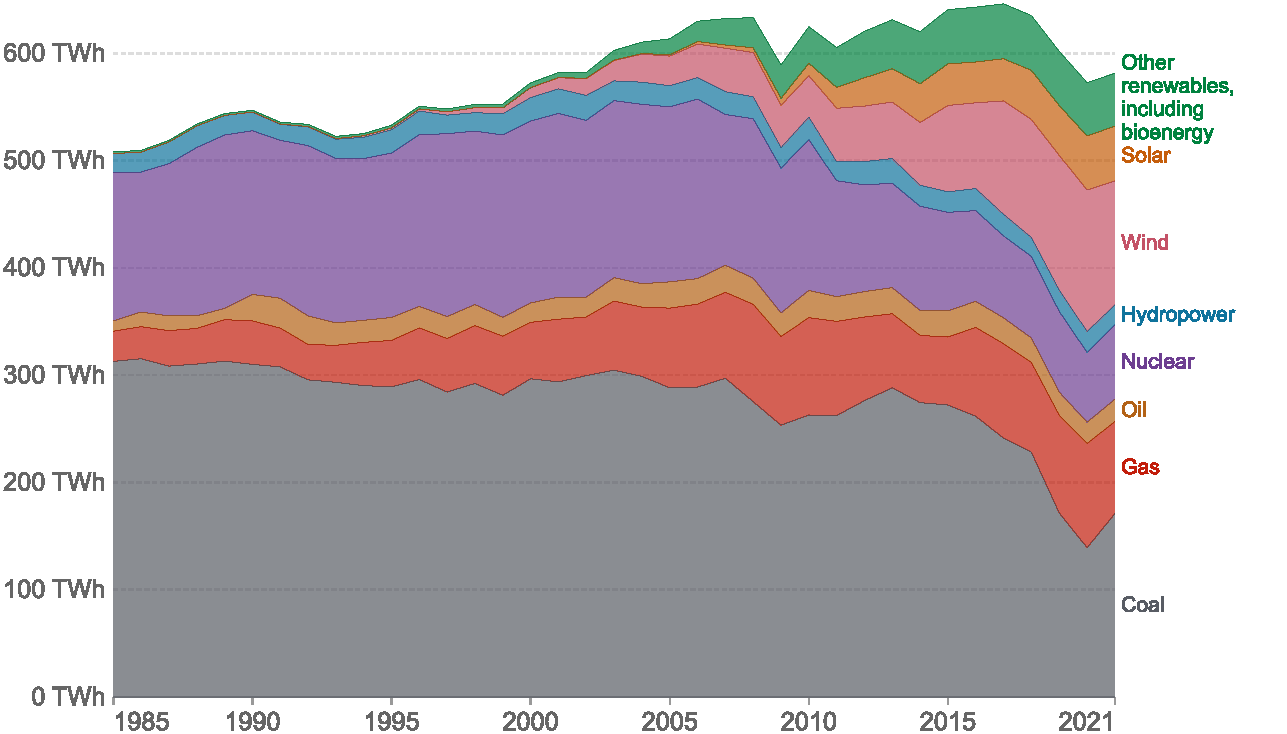
\includegraphics[width=0.45\textwidth]{Imágenes/Generacion de energía en Alemania.pdf}}    
  \hspace{3.5mm}
  \subfloat[Porcentajes de aporte de cada fuente de generación.]{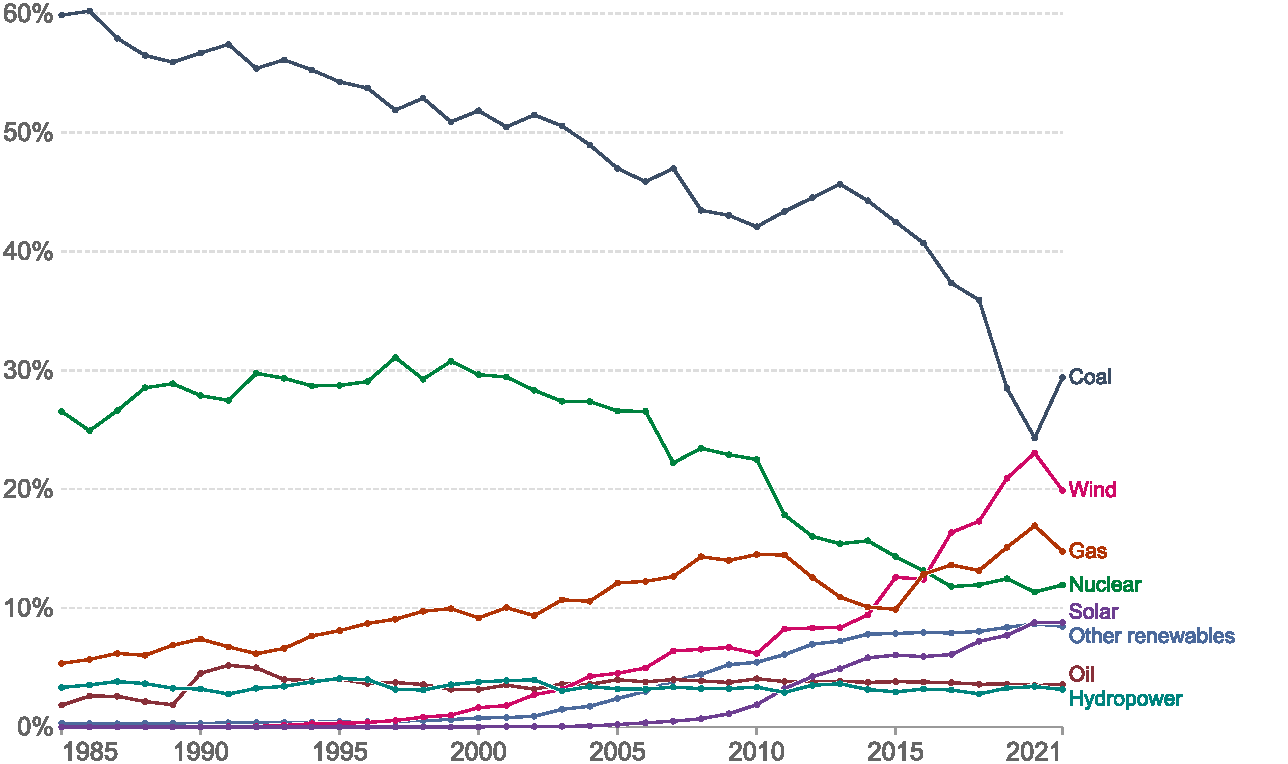
\includegraphics[width=0.45\textwidth]{Imágenes/Generacion de energía en Alemania en porcentaje.pdf}}
  \caption{Curvas de crecimiento de la generación de energías renovables.}
  \label{generacion-alemana}
\end{figure}

Por lo tanto, estos módulos de almacenamiento de energía son requeridos a distintos tamaños y con distintos fines, siendo algunos instalados en forma descentralizada (por ejemplo, en combinación con sistemas fotovoltáicos para aumentar su tasa de autoconsumo).

\subsubsection{Sistemas de potencia satelitales}

Los sistemas de potencia de satélites se han desplazado progresivamente hacia la tecnología de ión-litio desde los principios de los 2000s.  

A medida que el peso se convirtió en una cuestión clave de diseño para los satélites, la gran densidad másica de energía provista por la tecnologia Li-Ión aceleró su adaptación al principio de este siglo. Muy rápidamente, la transición ocurrió para los satélites de las órbitas geoestacionarias GEO (del inglés \emph{geostationary earth orbit}), órbita terrestre baja LEO (del inglés \emph{low earth orbit}) y la órbita terrestre media MEO (\emph{medium earth orbit}) gracias a las numerosas ventajas de las baterías Li-Ión, como su baja disipación térmica, autodescarga baja, y gran eficiencia. Para los fines de 2012, más de 200 satélites fueron lanzados mundialmente utilizando esta tecnología, y más del 99\% de los contratos satelitales refieren a las baterías Li-Ión en su diseño \cite{satellites}.

\begin{wrapfigure}{r}{0.45\textwidth}
  \vspace{-10pt}
  \begin{center}
    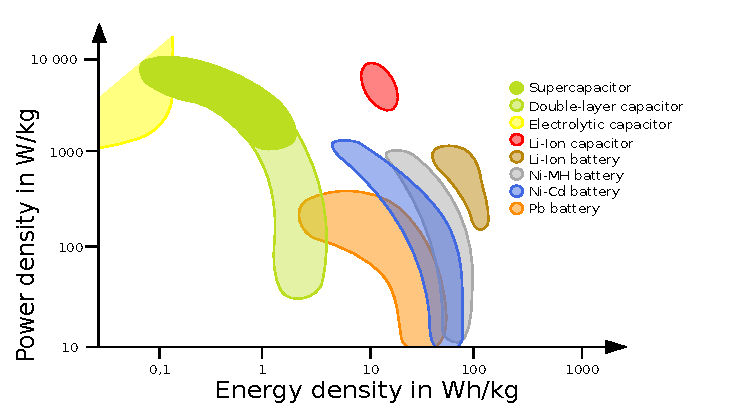
\includegraphics[width=0.44\textwidth]{Imágenes/Diagrama de Ragone.pdf}
  \end{center}
  \vspace{-15pt}
  \caption{Diagrama de Ragone.}
  \label{ragone}
\end{wrapfigure}

\subsection{Diferencias con los supercapacitores}

Como se ha visto, tanto las baterías como los supercapacitores son dispositivos de almacenamiento de carga con aplicaciones diversas, en las cuales ambos cumplen el rol de proveer energía. Sin embargo, los dos tienen características muy diferentes.

En la Figura \ref{ragone} puede observarse un diagrama de Ragone, el cual es utilizado para realizar comparaciones entre fuentes de almacenamiento. El eje horizontal indica la densidad másica de energía (en J/kg), lo que conceptualmente representa la capacidad de almacenamiento de energía. En cambio el eje vertical indica la densidad másica de potencia (en W/kg) y representa qué tan rápido puede ser entregada esa energía.

Aquí se puede observar la clara diferencia entre las baterías y los supercapacitores. Las baterías son capaces de almacenar mucha energía pero con una absorción y entrega de potencia mucho menos rápida que la de los supercapacitores. En cambio, los supercapacitores son capaces de entregar energía a una tasa órdenes de magnitud más alta, pero la cantidad de 
energía almacenada posible es limitada.

Estas diferencias pueden verse también en las aplicaciones mencionadas anteriormente para cada uno. En el caso de los supercapacitores, estos actuaban como búfer en situaciones de emergencia o con ventanas de tiempo cortas donde se requería una entrega importante de potencia. En cambio, el rol de las baterías de litio en los ejemplos dados era de almacenamiento de grandes cantidades de energía.

Es importante tener en cuenta que este diagrama no tiene en cuenta otras características intrínsecas de los módulos de almacenamiento, como su vida útil y su memoria.

\section{Sistemas híbridos de almacenamiento de energía}

Debido a sus características opuestas observadas en el diagrama de Ragone, las baterías y los supercapacitores se complementan muy bien, y por lo tanto la construcción de un sistema híbrido con ambos tipos de dispositivos presenta una gran flexibilidad a la hora de suministrar energía a aplicaciones móviles. En el caso de un sistema híbrido con baterías de litio y supercapacitores, el objetivo principal de las baterías es el de satisfacer la demanda de corriente, correspondiente a la potencia media demandada por el bus de continua \cite{estimacion}. Complementariamente, los supercapacitores son los encargados de lidiar con las variaciones abruptas de corriente que demande la carga.

La incorporación de un banco de supercapacitores en conjunto a la baterías de litio brinda además el incremento de la vida útil de la batería en un 300\%, ya que los picos de corriente serán entregados por el banco, lo que disminuye las exigencias de la batería.

Para formar este sistema híbrido, es necesario utilizar conversores electrónicos de potencia para poder ajustar los niveles de tensión de ambos dispositivos, y permitir que funcionen en conjunto. Estos tipos de conversores son analizados en el siguiente capítulo.   

\section{Resumen}

En este capítulo se desarrollaron las características de dos tipos de dispositivos que almacenan energía: los supercapacitores y las baterías de litio. Se presentaron sus mecanismos de funcionamiento, junto a algunas aplicaciones en las que se encuentran presentes.

Por último, se realizó una comparación de ambas con respecto a sus capacidades de almacenamiento de energía, y la rapidez con la que esta puede ser entregada. Este análisis de diferencias entre los dispositivos bajo estudio dió como conclusión que su operación en conjunto es capaz de formar un sistema híbrido con una gran flexibilidad bajo un amplio rango de operaciones.

\newpage